\label{ch:radiation}

\section{Equations of Radiation Hydrodynamics}

\subsection{Reference Frames}

\subsection{Angular Approximations / Moments}

\subsection{Closures}



\section{Hyperbolic System}



\section{Parabolic System}

\subsection{General Elliptic Solver}

For the gray radiation hydrodynamics system, we need to solve a
linear system that takes the form:
\begin{equation}
  \alpha \phi + \nabla \cdot \beta \nabla \phi + \gamma \cdot \nabla \phi = f
\end{equation}
(see Zhang et al., Eq. 45). 
We can discretize this for a cell-centered $\phi$ to second-order as:
\begin{align}
  \alpha_{i,j} \phi_{i,j} &+
  \frac{(\beta \nabla \phi)_{i+1/2,j} -
        (\beta \nabla \phi)_{i-1/2,j}}{\Delta x} +
  \frac{(\beta \nabla \phi)_{i,j+1/2} -
        (\beta \nabla \phi)_{i,j-1/2}}{\Delta y} \nonumber \\
  &+
  \gamma^{(x)}_{i,j} \frac{\phi_{i+1,j} - \phi_{i-1,j}}{2\Delta x} +
  \gamma^{(y)}_{i,j} \frac{\phi_{i,j+1} - \phi_{i,j-1}}{2\Delta y} = f_{i,j}
\end{align}
where we decompose the vector, $\gamma$ as $\gamma = \gamma^{(x)}\hat{x} + \gamma^{(y)}\hat{y}$.  Expanding the gradients:
\begin{align}
\label{eq:general_L}
\alpha_{i,j} \phi_{i,j} &+
  \frac{\beta_{i+1/2,j} (\phi_{i+1,j} - \phi_{i,j}) -
        \beta_{i-1/2,j} (\phi_{i,j} - \phi_{i-1,j})}{\Delta x^2} \nonumber \\
 &+
  \frac{\beta_{i,j+1/2} (\phi_{i,j+1} - \phi_{i,j}) -
        \beta_{i,j-1/2} (\phi_{i,j} - \phi_{i,j-1})}{\Delta y^2} \nonumber \\
  &+
  \gamma^{(x)}_{i,j} \frac{\phi_{i+1,j} - \phi_{i-1,j}}{2\Delta x} +
  \gamma^{(y)}_{i,j} \frac{\phi_{i,j+1} - \phi_{i,j-1}}{2\Delta y} = f_{i,j}
\end{align}

There are several different linear system algorithms people use to solve
these types of systems.  Since we have already developed a multigrid
solver, we will add equations of this type to the multigrid framework.

Defining $\tilde{\beta}_{i\pm1/2,j} \equiv \beta_{i\pm1/2,j}/\Delta x^2$,
$\tilde{\beta}_{i,j\pm1/2} \equiv \beta_{i,j\pm1/2}/\Delta y^2$,
$\tilde{\gamma}^{(x)}_{i,j} = \gamma^{(x)}_{i,j}/(2\Delta x)$,
and $\tilde{\gamma}^{(y)}_{i,j} = \gamma^{(y)}_{i,j}/(2\Delta y)$, we have
as an update to $\phi_{i,j}$,
\begin{align}
\label{eq:general_mg_smooth}
\phi_{i,j} = \frac{1}{D_{i,j}} \bigg [ f_{i,j}
  &-(\tilde{\beta}_{i+1/2,j} + \tilde{\gamma}^{(x)}_{i,j}) \phi_{i+1,j}
   -(\tilde{\beta}_{i-1/2,j} - \tilde{\gamma}^{(x)}_{i,j}) \phi_{i-1,j}
  \nonumber \\
  &-(\tilde{\beta}_{i,j+1/2} + \tilde{\gamma}^{(y)}_{i,j}) \phi_{i,j+1}
   -(\tilde{\beta}_{i,j-1/2} - \tilde{\gamma}^{(y)}_{i,j}) \phi_{i,j-1}
   \bigg ]
\end{align}
with
\begin{equation}
D_{i,j} = \alpha_{i,j} - \tilde{\beta}_{i+1/2,j} - \tilde{\beta}_{i-1/2,j}
                       - \tilde{\beta}_{i,j+1/2} - \tilde{\beta}_{i,j-1/2}
\end{equation}            

The remaining details of the multigrid solver are unchanged.  The boundary
conditions are implemented in the same way as done for Poisson's equation.
For radiation, we will need to implement inhomogeneous boundary conditions,
which we can do via the ghost cell filling using Eqs.~\ref{eq:bc_inhomo_dir}
and \ref{eq:bc_inhomo_neum}.  Note that because of this general form
of the equation, it is no longer simple to do the boundary charge method
described in \S~\ref{sec:multigrid:other}, so we must modify the ghost
cell fill routines explicitly.

The only changes to the core solver are in the smoothing function, which
implements Eq.~\ref{eq:general_mg_smooth} and in the residual, which
constructs our operator as discretized in Eq.~\ref{eq:general_L}.

To test this solver out, we can define a test problem by picking functional
forms of $\alpha$, $\beta$, and $\gamma$, and a solution, $\phi$, with
desired boundary conditions and find the resulting $f$ matching:
\begin{equation}
  \label{eq:general_elliptic}
\alpha \phi + \nabla \cdot (\beta \nabla \phi) + \gamma \cdot \nabla \phi = f
\end{equation}
Let's find a set of coefficients and righthand side for which
\begin{equation}
\phi = \cos(\pi x/2) \cos(\pi y/2)
\end{equation}
is a solution on $[0,1]\times[0,1]$.  This would satisfy the Dirichlet
boundary conditions:
\begin{align}
\phi |_{x=0} &= \cos(\pi y/2) \\
\phi |_{x=1} &= 0 \\
\phi |_{y=0} &= \cos(\pi x/2) \\
\phi |_{y=1} &= 0
\end{align}
For the coefficients, we choose:
on  with homogeneous Dirichlet boundary conditions.  We
use
\begin{align}
\alpha &= 10 \\
\beta  &= xy+1 \\
\gamma &= \hat{x} + \hat{y}
\end{align}
This gives
\begin{align}
  \label{eq:general_elliptic_rhs}
f = &- \frac{\pi}{2} (x + 1)
   \sin{\left (\frac{\pi y}{2} \right )} \cos{\left (\frac{\pi x}{2} \right )}
 - \frac{\pi}{2} (y + 1)
   \sin{\left (\frac{\pi x}{2} \right )} \cos{\left (\frac{\pi y}{2} \right )}
    \nonumber \\
   &+ \left(10- \frac{x y+1}{2} \pi^{2}\right)
    \cos{\left (\frac{\pi x}{2} \right )} \cos{\left (\frac{\pi y}{2} \right )}
\end{align}

Figure~\ref{fig:general_mg_converge} shows the convergence of multigrid
for this problem, and figure~\ref{fig:general_mg_solution} shows the solution.
We see second order convergence, as expected with this discretization.

\begin{figure}
  \centering
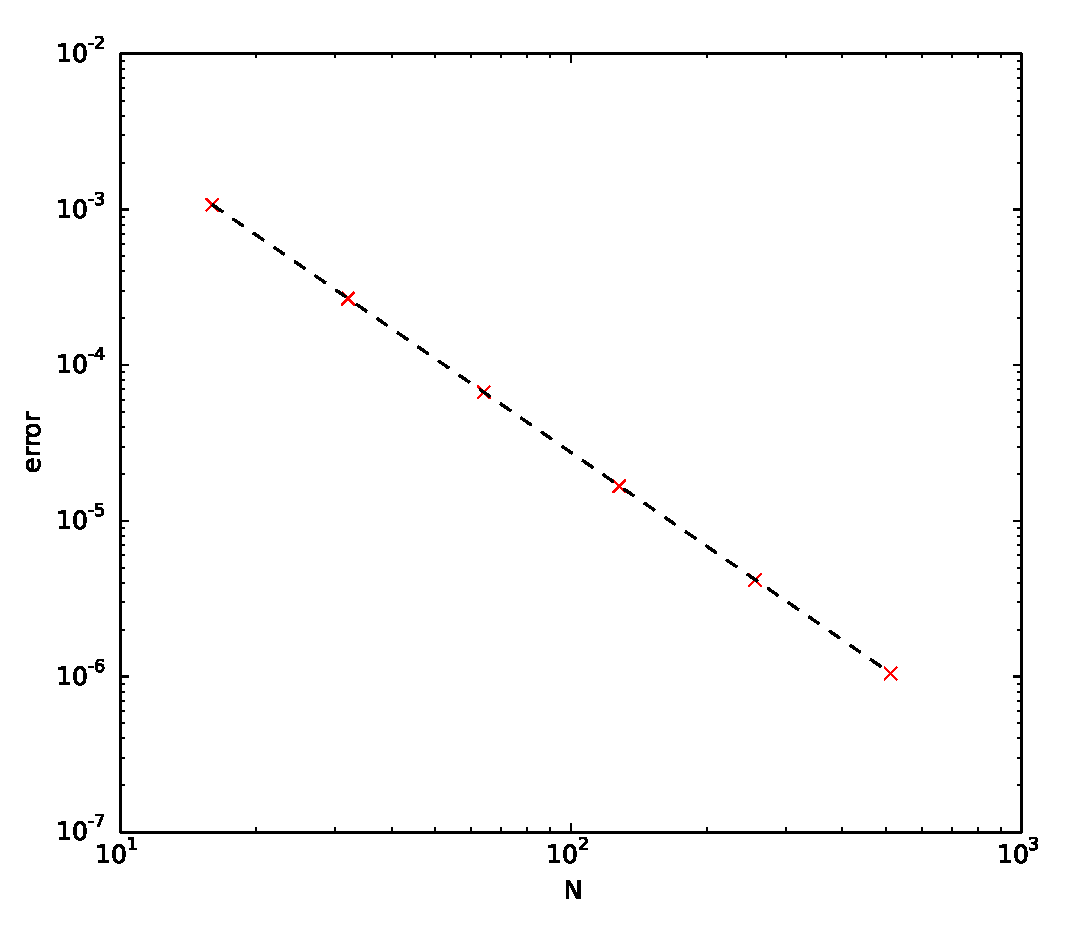
\includegraphics[width=0.6\linewidth]{mg_general_inhomogeneous_converge}
\caption[Convergence of the general elliptic multigrid
  solver]{\label{fig:general_mg_converge} Convergence of the multigrid
  solver on our test problem $\alpha \phi + \nabla \cdot (\beta \nabla \phi) +
  \gamma \cdot \nabla \phi = f$ with inhomogeneous Dirichlet boundary conditions.}
\end{figure}

\begin{figure}
  \centering
  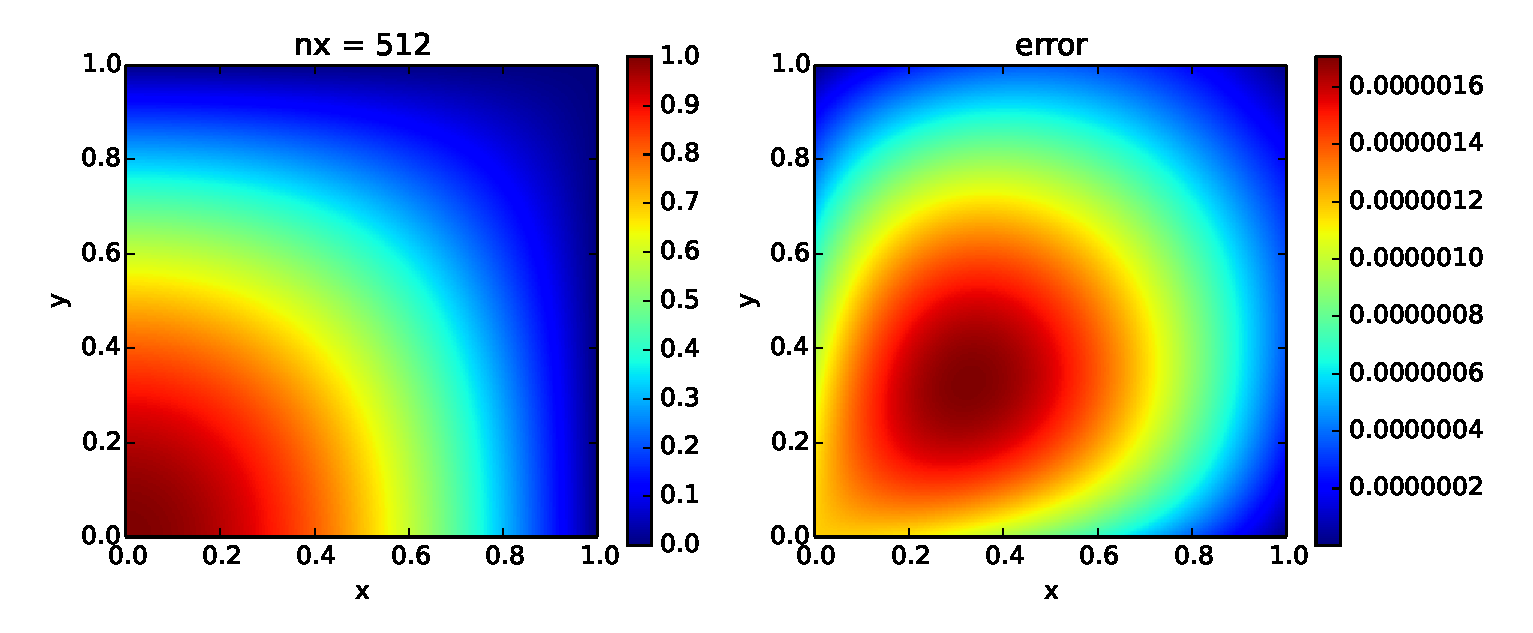
\includegraphics[width=\linewidth]{mg_general_inhomogeneous_test}
  \caption[Solution of a general elliptic equation]
          {\label{fig:general_mg_solution} The solution to our general
            elliptic text problem, Eqs.~\ref{eq:general_elliptic} to
            \ref{eq:general_elliptic_rhs} with inhomogeneous boundary
            conditions on a $512^2$ grid.  This test can be run in \pyro\
            {\tt multigrid/test\_mg\_general\_inhomogeneous.py}.}
\end{figure}
